\documentclass[12pt,a4paper,twoside,openright]{report}
\usepackage{algpseudocode}		% ambienti per la scrittura di algoritmi
\usepackage{algorithm}			% 

\usepackage{epsfig}						% figure eps
\usepackage{graphicx}					% figure qualsiasi
\usepackage{amsmath,amsfonts,amsthm}		% package di scrittura matematica
\usepackage{amssymb}
\usepackage{psfrag}
\usepackage{fancyhdr}
\usepackage{url}
\usepackage{array}
\usepackage{subfigure}
\usepackage{lscape}
\usepackage{colortbl}
\usepackage{alltt}
\usepackage{tabularx}
\usepackage[english]{babel}
\usepackage[nottoc]{tocbibind}
\sloppy
\raggedbottom

\linespread{1.3}
\renewcommand{\baselinestretch}{1.3}

\makeatletter
\def\cleardoublepage{\clearpage\if@twoside \ifodd\c@page\else
\hbox{}
\vspace*{\fill}
\begin{center}
%This page intentionally contains only this sentence.
\end{center}
\vspace{\fill}
\thispagestyle{empty}
\newpage
\if@twocolumn\hbox{}\newpage\fi\fi\fi}
\makeatother

%\newcites{wb}{Web References}

%------------------------------------------------------
% Impostazioni per il controllo sillabazione vedove/orfane ect..
%
% \looseness=1 o \looseness=-1 prima di un paragrafo per
% allungarlo o accorciarlo di una riga
%------------------------------------------------------

\lefthyphenmin=4
\righthyphenmin=4
\tolerance=1000
\hyphenpenalty=100
\emergencystretch=1 cm

\widowpenalty=5000
\clubpenalty=2500

%--------------------------------------------------------
% impostazioni per la dimensione delle pagine
%--------------------------------------------------------
\renewcommand{\headrulewidth}{0.5pt}
\hoffset=-15mm
%\topmargin=0mm
\headheight=15pt
\textwidth=140mm
\headsep=5mm
\voffset=-5mm
%\hsize=13cm
%\textwidth=164mm
\textheight=230mm
\evensidemargin=25mm
\oddsidemargin=25mm
%\marginparwidth=0mm

\renewcommand{\abovecaptionskip}{0pt}
\renewcommand{\belowcaptionskip}{0pt}

%--------------------------------------------------------------
%impostazione headers
%--------------------------------------------------------------
\pagestyle{fancy}
%\addtolength{\headwidth}{\marginparsep}
%\addtolength{\headwidth}{\marginparwidth}
\renewcommand{\chaptermark}[1]{\markboth{#1}{}}
\renewcommand{\sectionmark}[1]{\markright{\thesection\ #1}}
\fancyhf{}
\fancyfoot[LE,RO]{\bfseries\thepage}
\fancyhead[RO]{\bfseries\rightmark}
\fancyhead[LE]{\bfseries\leftmark}
\fancypagestyle{plain}{%
\fancyhead{} % get rid of headers
\fancyfoot{}
\renewcommand{\headrulewidth}{0pt} % and the line
}

\newenvironment{myverse}
{\small}
{}

\newenvironment{myabstract}{%
  \begin{center}%
    \null\vfil
    \bfseries \abstractname
  \end{center}}%
{\par\vfil\null}

\newcommand{\newparagraph}{\noindent\\}

\begin{document}

\pagenumbering{roman}
\setcounter{page}{1}
\pagestyle{empty}

%--------------------------------------------------------------------------------
% include title page
%--------------------------------------------------------------------------------
\begin{titlepage}
\vspace*{-2.5cm}
\bfseries
\begin{center}
  \LARGE
  Politecnico di Milano\\
  \Large
  Computer Science and Engineering\\


\psfig{file=images/logopm,width=4cm}

\begin{large}
Scuola di Ingegneria Industriale e dell'Informazione\\
Computer Science and Engineering\\
\end{large}

\vspace{2.0cm}
\begin{Large}
Avoiding CRUD operations lock-in in NoSQL databases: extension of the CPIM library
\end{Large}  
\end{center}

\vspace*{4cm}
\large
\begin{flushleft}
\hspace{-2cm}  Advisor: Elisabetta DI NITTO\\
\hspace{-2cm}  Co-Advisor: Marco SCAVUZZO\\
\end{flushleft}
\vspace*{1.5cm}

\hspace{6cm}
\parbox{10cm}{
    \begin{tabular}{ll}
         Master thesis by: & \\
         Fabio ARCIDIACONO & matr. 799001\\
    \end{tabular}
}

\vspace*{2cm}
\begin{center}
  Academic Year 2013-2014
\end{center}

\end{titlepage}
\cleardoublepage

%--------------------------------------------------------------------------------
% ringraziamenti
%--------------------------------------------------------------------------------
\thispagestyle{empty}

\chapter*{Ringraziamenti}
Ringrazio la professoressa Di Nitto e Marco Scavuzzo per avermi dato la possiblit\`{a} di svolgere questo lavoro di tesi e per l'aiuto e la disponibilit\`{a} con cui mi hanno seguito in questi mesi.

\noindent Ringrazio la mia famiglia per avere sempre assecondato le mie scelte e non avermi mai fatto mancare il loro sostegno.
 
\noindent Ringrazio Crizia per essere un costante punto di riferimento nella mia vita e per avermi sostenuto durante tutto il percorso.

\noindent Ringrazio gli amici per la pazienza con cui mi hanno sopportato in questi anni.

\noindent Infine voglio ringraziare Lorenzo e Riccardo, che hanno reso questi due anni di magistrale un percorso memorabile.
 
\noindent \textit{We were stuck in a blender and now we're saving lives!}

\begin{flushleft}
Milano, 1 Aprile 2015
\end{flushleft}

\begin{flushright}
\emph{Fabio.}
\end{flushright}

\cleardoublepage

\pagestyle{fancy}
\renewcommand{\contentsname}{Table of Contents}%

%--------------------------------------------------------------------------------
% include the abstract in italian
%--------------------------------------------------------------------------------
\chapter*{Estratto}
\input{content/estratto}

%--------------------------------------------------------------------------------
% include the abstract in english
%--------------------------------------------------------------------------------
\chapter*{Abstract}
\input{content/abstract}

%--------------------------------------------------------------------------------
% talbe of contents
%--------------------------------------------------------------------------------
\tableofcontents
\cleardoublepage
\listoffigures
%\listoftables
 
\pagenumbering{arabic}

\setcounter{page}{1}

%--------------------------------------------------------------------------------
% introduction
%--------------------------------------------------------------------------------
\chapter{Introduction}
\label{chap:one}
In the last few years, due to the advent of Web 2.0, more and more data becomes available, generated by a growing multitude of people. The nature of this kind of data is intrinsically unstructured and comes in a volume that traditional data management techniques are no more affordable to guarantee modern application requirements.
In this scenario, NoSQL databases have emerged over traditional DBMS as a more suitable alternative to handle those new kinds of data.

\noindent NoSQL databases try to address the new applications requirements in terms of: fault tolerance, availability across distributed data sources, scalability and consistency, in different ways, proposing different properties and characteristics. 
Each NoSQL database thus provides to its users a different API interface tailored to exploit the specific characteristic that the NoSQL offer.

\noindent The lack of a common language for NoSQL databases, require, when developing an application, a clear understanding of the available NoSQL solutions, to be able to choose the right technology for the application requirements. However, during the life cycle of the application, changing the adopted NoSQL technology, maybe due to requirements changes, may become a problem. This problem is known as \textit{vendor lock-in}.  

\noindent To mitigate the problem, this work proposes an extension of the CPIM library, which already try to address the vendor lock-in problem in PaaS environments, in order to provide to the user a way to abstract from the specific NoSQL technology used to store the data.
Many solutions has been proposed by both communities and industry, in defining a common way to access different NoSQL technologies. We propose to use the one that seems to get most interest, especially by the industry, which is the use of the JPA interface. With this objective we integrate Kundera, an ORM for NoSQL databases based on the JPA standard interface in the NoSQL service of the CPIM library, furthermore we develop new extensions for Kundera to support the database currently supported by CPIM.
The complexity of using NoSQL databases is moved inside Kundera clients and this permit to the user to access several NoSQL technologies by using both a standard language, which is JPQL (a SQL-like language), and a well known interface among Java developer, the JPA interface.

\noindent To achieve complete portability, both of the code and of the stored data, this work also propose the integration, in the CPIM library, of the migration and synchronization system \textit{Hegira}. This permit to the user a way of moving its data from a NoSQL technology to another without experiencing application down time, and thus be able to change the NoSQL technology without the need of re-engineering the application.
 
\section*{Original Contributions}
This work include the following original contributions:
\begin{itemize}
\item two brand new Kundera clients, one for Google Datastore and one for Azure Tables;
\item the support, for the  NoSQL service of CPIM library, for the interaction with the migration system \textit{Hegira}, both for data synchronization and migration; 
\end{itemize}

\section*{Outline of the Thesis}
This thesis is organized as follows: 
\begin{itemize}
\item In Chapter \ref{chap:sota} is described the evolution of NoSQL. As a first introduction is discussed why in this years this technology have emerged over SQL solutions and what are the main differences among those technology, the second part aims to underline the lack of a common language for NoSQLs in contrast to DBMS in which SQL exists.
\item In Chapter \ref{chap:ps} we analyze the current available technologies for NoSQL databases and propose a work for extending the CPIM library to make its interaction with NoSQL world even easier and much more extensible. Furthermore we analyze the requirements of modern web application motivating the choice of integrating in the CPIM NoSQL service a mechanism of data migration.
\item Chapter \ref{chap:kundera} is dedicated to the develop of the two Kundera client extension that have been developed in order to support Google Datastore and Azure Tables that will be then used in CPIM as adapters for the relative database.
\item In Chapter \ref{chap:cpim} is presented the work made on CPIM. As a first step is described a modification in the CPIM NoSQL service aimed to integrate Kundera as unique persistence layer for NoSQL access using the standard JPA interface, the library was previously using several different JPA implementation one for each of the supported databases. Furthermore is discussed the extension of CPIM to include an interaction with the migration system \textit{Hegira}.
\item In Chapter \ref{chap:eval} are described the various tests that have been performed on the developed Kundera extensions, to guarantee the correctness of the operation and to provide a measurement of performance. Moreover is presented a test application developed to be able to test the migration of the data generated through the CPIM library through the NoSQL service.
\item In Chapter \ref{chap:conclusions} draws the conclusions on the entire work and proposes some possible future works.
\end{itemize}



%--------------------------------------------------------------------------------
% State of the art
%--------------------------------------------------------------------------------
\chapter{State of the art}
\label{chap:soa}
\section{Introduction}
Introduzione agli argomenti trattati nel capitolo, dalle 4 alle 10 righe.

\section{Summary}
Riassunto del capitolo

%--------------------------------------------------------------------------------
% Problem setting
%--------------------------------------------------------------------------------
\chapter{Problem setting}
\label{chap:ps}
\section{Introduction}
In this chapter we expose the motivations that lead us to conduct this work, in particular, we analyze the current problems in the NoSQL service implementation of the CPIM library and propose a solution to address them and, at the same time, increasing the number of NoSQL database supported by the library.
\noindent Furthermore, we will discuss why we decided to include the possibility for the CPIM library users to be able to migrate and synchronize data, across databases, by means of a migration system called \textit{Hegira}.

\section{CPIM library extension}
Cloud Platform Independent Model (CPIM) \cite{thesis:cpim} is a Java library built in order to make Java developers able to abstract their application logic from the specific PaaS Provider on which the application will actually be deployed.



\subsection{CPIM NoSQL service}
The CPIM library uses various implementation of the JPA interface to ease the communication with different NoSQL databases:
\begin{itemize}
\item Google Datastore is supported by means of the Google JPA implementation around Datastore API;
\item Azure Tables is supported through \textit{jpa4azure} a third party implementation of the JPA interface for Tables;
\item Amazon Simple DB is supported through \textit{simpleJPA} a third party implementation of the JPA interface for Simple DB.
\end{itemize}
\noindent By choosing the cloud provider inside the \textit{configuration.xml}, the library knows, at run-time, which interface should be used for the service and this holds also for the NoSQL service. Hence to use Google Datastore as NoSQL database, Google must be selected as cloud provider.

\noindent The aim of CPIM is to offer to the user a way of writing cloud application in a provider-independent fashion, to be able to migrate the application from a provider to another without the necessity of re-engineer the application. For the NoSQL service this is achieved by meas of the JPA interface that, beside the fact that is is not a standard for accessing NoSQLs, many projects came into play trying to bring the benefit of the JPA interface also in the NoSQL world.

\newparagraph As discussed in chapter \ref{chap:sota}, the use of the JPA interface in defining a common interface for accessing NoSQL databases is a solution widely adopted, thus the choice of using the JPA as abstraction layer for the NoSQL service in the CPIM is a valuable choice. 
However the current implementation have significant problem:
\begin{enumerate}
\item[\textbf{P.1}] the application code written to interact with the NoSQL service is not interoperable and thus, the user is required to modify the application code in order to be able to move the application to a different cloud provider.  
\end{enumerate}
\noindent Moreover the NoSQL service suffer of some limitations too:
\begin{enumerate}
\item[\textbf{L.1}] the choice of the NoSQL database is strictly bind to the selected cloud provider; 
\item[\textbf{L.2}] even if the selection of the NoSQL database would be possible, the number of supported NoSQL database is very limited.
\end{enumerate}

\noindent For \textbf{P.1}, the problem reside in the fact that for each of the currently supported database, has been found and integrated into CPIM, a specific implementation of the JPA interface. Even through JPA is a well defined standard, not every JPA provider follows strictly the specification and thus, different provider can behave differently while persisting the same entities, since they interpret differently the semantic of some JPA annotation.

\noindent An example of this problem is how Collection fields are currently handled in CPIM. In the Google JPA implementation for Datastore and in the JPA implementation for Amazon SimpleDB, Collection fields are handled correctly, with respect to the JPA specification, thought the \texttt{@ElementCollection} annotation, while, in the JPA implementation for Azure Tables, Collection fields needs to be annotated with the \texttt{@Embedded} annotation. This require a modification of the code and thus eliminates the effort of CPIM in achieving code portability among PaaS.

\newparagraph As regards \textbf{L.1} and \textbf{L.2}, we would like to  give to the user the ability to persist data in the database that best fit his requirements. For example if the user application will generate data that should be processed with Hadoop, the best solution is to store those data in an HBase instance since its integrate easily in Hadoop. Therefore we want to make the user able to persist different entities in different datastore based on his needs and without the limitation of a specific NoSQL technology.

\subsection{Proposed solution}
The proposed solution is mainly about the integration of Kundera, a JPA compliant ORM for NoSQL databases, as unique persistence layer for the NoSQL service. This integration will be useful to solve the problems and mitigte the limitation outlined as follow:
\begin{itemize}
\item since Kundera will be the unique persistence provider for the library we will relay only on one implementation of the JPA interface overtaking in this way, the problem \textbf{P.1}, related to different interpretation of the JPA annotation, and thus achieving complete portability of the code of the application model since no code modifications are required to work with different NoSQL database through Kundera;
\item the integration of Kundera permits a redesign of the NoSQL service aimed to decouple the chosen PaaS provider and the NoSQL technology overcoming limitation \textbf{L.1}, by giving to the user the ability of deciding which technology is more suitable for his needs. Furthermore exploiting the polyglot-persistence provided by Kundera, the user will be able to persist entities within different NoSQL databases at the same time, simply by defining accordingly the persistence unit in the \textit{persistence.xml} file;
\item choosing Kundera as persistence layer we can actually take advantage of the already developed extension for many different NoSQL databases, adding as a result the support of those database to CPIM, and thus overcoming the limitation \textbf{L.2}.
\end{itemize}

\noindent There are many reasons why we choose to use Kundera as persistence provider for the NoSQL service of the CPIM library. The main reason is that Kundera, through the use of the JPA interface will permit to the user to handle the complexity of NoSQL databases with expertise he already uses for SQL systems. Furthermore Kundera is in the field from 2010 and thus have a big and active community, built in many years of activity, and has been used successfully in some production environment.

\noindent The only drawback is that Kundera does not support any of the NoSQL datastore currently supported by CPIM. Fortunately Kundera have, as its primary goal, to make the library as much extensible as possible, to let developers build their own client around new NoSQL technologies. The solution will thus be to develop the needed extensions for Kundera.

\newparagraph The work on the CPIM NoSQL service will thus require:
\begin{itemize}
\item the integration of Kundera as the unique persistence provider in the NoSQL service of CPIM;
\item the development of two brand new Kundera extensions, one for Google Datastore and one for Azure Tables.
\end{itemize}

\section{Data migration}
NoSQL technologies do not offer a common querying language to interact with them, as SQL does for RDBMS. Furthermore, NoSQLs offer a simpler interface with respect to RDBMS and each of them exposes a proprietary API tailored to the specific database needs. This requires to interact with NoSQL databases at a lower level of abstraction, moving a good amount of developing effort toward the user.
Given the amount of NoSQL solutions available nowadays \cite{online:nosql-database.org}, and this low-level approach in using such technologies, a company that want to adopt a NoSQL solution to manage its data, finds itself locked to the chosen technology. 
For this reasons while NoSQL solutions can be appetible to industry, the high costs of application re-engineering and the necessity of investments on qualified personnel, disrupt the adoption of such technologies.

\noindent The CPIM library can mitigate this vendor lock-in problem by giving to the user the freedom to choose the NoSQL solution that best fit its application requirements and, furthermore, by using the JPA interface, gives the possibility to interacts with NoSQL databases with expertise that companies already have.

\noindent However when a company actually faces the problem of changing the storage solution for its data, even if the application, through frameworks like CPIM, permits effortless code portability, data migration from the old storage to the new one became a huge problem. 

\newparagraph Data migration has became a key feature in modern IT, there exists many reasons to move data from one storage to another: for load balancing, system expansion, failure recovery, etc.

\noindent Typical migration solutions involve applications stop to move the data offline and restart the application when the process has been completed, to guarantee the correctness. On the other hand, modern computer systems are expected to be up continuously and thus even planned downtime to accomplish system reconfiguration is becoming unacceptable \cite{paper:hitachi}.

\begin{figure}[tbh]
  \centering
  \includegraphics[width=13cm]{images/hitachi_survey}
  \caption{Perceived risk in data migration \cite{paper:hitachi} }
  \label{fig:cpim-nosql}
\end{figure}

\noindent However migrating data between database without causing application downtime brings several new problems such as data synchronization between the two involved systems.

\subsection{Hegira integration}
To mitigate those problems we want to extend the CPIM library to make it able to interact with \textit{Hegira} a migration system able to perform interoperable data migration and synchronization across column-based NoSQL databases \cite{paper:modaclouds-deliverable}. \textit{Hegira} is already able to migrate data offline, but in many cases this solution is not acceptable since this requires to turn off the application for a period of time that depends on the volume of data that needs to be migrated towards the new database. 
Downtime costs and risks of data loss can be problematic so, \textit{Hegira} was extended to be able to perform a live-migration of the data by keeping them synchronized on the source and the destination database.
This feature needs to be exploited at application level and thus we decided to embed it inside the CPIM NoSQL service, in order to make it as transparent as possible to the user.

\noindent The CPIM library needs to be aware of the state of both the synchronization and migration systems and acts accordingly intercepting user operation and sending data manipulation queries (DMQ) to the migration system which is in charge of keeping the data consistent across the replicated databases.

\noindent The result of such integration in the CPIM library will be the ability of the user to migrate data from a NoSQL storage to another, while the application is running, and still be able to read the data on the new system without modifying the application code

%--------------------------------------------------------------------------------
% Kundera extension
%--------------------------------------------------------------------------------
\chapter{Kundera extension}
\label{chap:kundera}
\section{Introduction}
In this chapter will be presented briefly the Kundera modular architecture, the way in which Kundera is supposed to be extended, the problems occurred in the process and how the community helped in achieving the result.
Then are discussed the detail of the two Kundera extension developed, in section \ref{sec:kundera-datastore} the one for Google Datastore and in section \ref{sec:kundera-table} the one for Azure Table.

\section{Overview of Kundera}
Kundera \cite{online:kundera} is an implementation of the JPA interface that now supports various NoSQL datastore. It supports by itself cross-datastore persistence in the sense that its allows an application to store and fetch data from different datastores.
Kundera provides all the code necessary to implement the JPA 2.1 standard interface independently from the underlying NoSQL database. 

\newparagraph The currently supported NoSQL databases are:
\begin{itemize}
\item Oracle NoSQL (versions 2.0.26 and 3.0.5)
\item HBase (version 0.96)
\item MongoDB (version 2.6.3)
\item Cassandra(versions 1.2.9 and 2.0.4)
\item Redis (version 2.8.5)
\item Neo4j (version 1.8.1)
\item CouchDB (version 1.0.4)
\item Elastic Search (version 1.4.2)
\end{itemize}

\begin{figure}[tbh]
  \centering
  \includegraphics[scale=0.5]{images/kundera_architecture}
  \caption{Kundera architecture}
  \label{fig:kundera_architecture}
\end{figure}

\newparagraph The architecture of Kundera is shown in Figure \ref{fig:kundera_architecture}. The figure highlights the fact that the user application interacts with Kundera simply by exploiting the standard JPA interface implemented in the Kundera-Core.
Kundera-Core, each time an operation need to be executed on the underlying database, delegates the operation to the appropriate \texttt{Client} creating it through a \texttt{Client Factory} if it does not exists yet.

\subsection{Kundera's Client Extension Framework}
Kundera try to offer a common way to interacts with NoSQL databases through a well defined interface and as on open source project make other developers able, if interested, in using and extending it adding support to other datastore.
Is so available a Client Extension Framework descripted in the Kundera wiki which provides a short introduction on how Kunders clients should work and provides the interfaces and classes that should be developed in order to make the client work properly.

\newparagraph Basically to build a new Kundera client, these are the blocks to be developed:
\begin{itemize}
\item the \texttt{Client}, which is the gateway to CRUD operations on database, except for queries;
\item the \texttt{Client Factory}, which is used by Kundera to instantiate the Client;
\item the \texttt{Query implementor}, which is used by Kundera to run JPA queries by invoking appropriate methods in Entity Readers;
\item the \texttt{Entity Reader}, which is used by Kundera to translate the queries into correct client
method calls;
\item optionally the \texttt{Schema Manager}, to support automatic schema generation.
\end{itemize}

\subsection{Approaching the extension}
It all seems quite simple but the problem is that the documentation is actually outdated. 
Two were the main problem in understaing what to do and how, firstly it turns out that the required interfaces are actualy a little different and also are the required methods
secondary, and slightly more time consuming, is that no hints nor documentation are given on the structure and informations carried by the methods arguments.
The arguments carrys data structures containing informations organized in the kundera metamodel which is the implementation of the JPA metamodel that contains all the information associated (throug annotations) to a class or a field.

\newparagraph Due to those problems and to shrink the developing time, the solution was to write on the Kundera google group page to ask the community for more updated infos about Kundera extension.
Briefly an answer has come and I've started a conversation with one of the developers of Kundera who helped me giving the updated informations for the Kundera's Client Extension Framework and tell me to look forward to the other client implementation for some examples. 
Thanks to the updated information it turns out that the \texttt{Entity Reader} was unnecessary and all the translation from JPA queries to datastore specific queries and their executions should be done in the \texttt{Query Implementor}.  

\noindent At this point since no answer were given about the Kundera metamodel, the most valid solution was to approach the extesion as a test driven development, so, looking at the tests code of the other clients, I've writed a set of unit tests one for each feature.
With the tests failing and studyng the code of the other Kundera clients was then possible to reverse engineer the arguments thath were not documented and thus be able to develop the new extensions.

\newparagraph Unit tests are analyzed in detail in the chapter \ref{chap:eval}.

\section{Developing client extensions}
Have been developed two different extension for Kundera, the first one for Google Datastore and the second one for Azure Table.
After a first difficulty in figuring out how the extension have to be carried out, a main structure has been defined so the two projects have many parts in common. 
In the following sections the extensions are presented separately, the concepts are introduced as they are encountered and will be referenced further on if necessary specifying the differences if any.

\subsection{Google App Engine Datastore client}
\label{sec:kundera-datastore}
The first extension that has been faced is the one for Google App Engine (GAE) Datastore \cite{online:datastore} the NoSQL solution available in the App Engine runtime, is a key-value storage build on top of Google BigTable.

\subsubsection{JPA identifier}
In Google Datastore the most basic unit that can be stored is an Entity which is identified by a Key and composed of Properties.
Entities Keys contains various information about the entity itself:
\begin{itemize}
\item the entity Kind, which is used to group entities of the same type;
\item an entity identifier, used to distinguish entities of the same type;
\item an optional parent entity. 
\end{itemize}
Inspired by the Google JPA implementation on Datastore the idea was to use the Java class representing the datastore Key as indentifier for the POJO but unfortunately this was not possible since Kundera support only a pre defined set of Java datatypes.

\newparagraph The adopted solution is to handle the key internally, each time an opertion is required on Datastore the key relative to the entity is builded, the key Kind is directly mapped to the table name and the Key identifier is the user defined id in the \texttt{@Id} annotation.

\noindent IDs can be specified by the user or automatically generated, there are three possibilities:
\begin{itemize}
\item \texttt{@Id} annotation on a \texttt{String} type field
\item \texttt{@Id} annotation on a \texttt{Long} type field
\item \texttt{@Id} annotation on a primitive \texttt{long} type field
\end{itemize}
For each case the ID can be user specified before the persist operation but in case of ID auto-generated the field must be of type \texttt{String} and the generated ID will be a string representation of a random java \texttt{UUID}.

\noindent Auto-geenerated ID are supported by Kundera thorugh \texttt{@GeneratedValue} with \texttt{AUTO} or \texttt{TABLE} strategy, only \texttt{AUTO} strategy is supported. 
It was not possible to use the Datastore API to generate IDs since is necessary to know the Kind of the entity to be persisted but neither the \texttt{AUTO} strategy nor the \texttt{TABLE} one provides this infomation at generation time.

\subsubsection{Consistency}
In Datastore entities are organized in Entity Groups based on their Ancestor Path, the ancestor path is a hierarchy containing the keys of the entities which are parents of the given one and thus in the same entity group.

\noindent Consistency is managed through Entity Groups and so by defining the ancestor paths, entities within the same Entity Groups are managed in storng consistency, eventual consistency is used otherwise.

\noindent Datastore provide the possibility to create Ancestor path by defining entities parent to other entities and is basically a task left to the user, no automated sorting or guessing is provided. Other wrapper around Datastore low-level API also leave this to the user, for example in Objectify \cite{online:objectify} the developer make use of an \texttt{@Parent} annotation that make the user able to specify the Ancestor Path.
Since JPA is well defined and adding such annotation will break the standard the only alternative way is trying to automatic guess the ancestor path.

\newparagraph Relationsips are clearly a good point where found information for guessing if two entitiy kind can be hirearchically related, so for each type of relation must be defined what solution can be adopted.
\begin{itemize}
\item for \textbf{One to Many} and \textbf{One to One} relationships, since there's an owning side, the owning entity can be used as parent for every related entity. 
\item \textbf{Many to One} can be skipped since are the inverse of \textbf{One to Many} so such related entities should be already organized. 
\item for \textbf{Many to Many}, since the realtionship is handeled through a join table, it does not make sense to relate the entities involved.
\end{itemize}

\noindent Also if possible this guessing was not done in the extension for two main reasons:
\begin{enumerate}
\item entities are not require to have a single relationship
\item entities with a parent require the parent Key to be universally identified
\end{enumerate}
So for the first reason is impossible, unless asking to the user, to decide which relation use to hierarchically organize entities, furthermore for the second reason when declaring a entity parent to another is always necessary to know the Key of the parent (and thus its Kind and identified) beside the Key of the entity itself to be able to retrieve it from Datastore and for how Kundera is structured this information is not available during find operation in which Kundera provides only the table name, the identifier and the entity class.

\newparagraph For those reasons was not possible, without causing errors, to automatically guess ancestor paths through JPA relationships or make the user able manage them directly through a specific annotation.
Each Kind is persisted as a root Kind and so each entity is stored in a separated entity group identified by its Kind (the name of the JPA table associated to the entity).

\subsubsection{JPA relationships}
All the JPA supported relationships \cite{book:projpa2} has been implemented in the client and  have been implemented like they would be in a RDBMS system.
So for \textbf{One to One} and \textbf{One to Many} relationships on the owning side of the relationships a \textit{reference} to the non-owning side entity is saved.

\noindent For \textbf{Many to One} relationships there would be two solutions:
\begin{itemize}
\item persist a list of \textit{references} tp the related entities;
\item do not persist anything within the entity and fill the relationship with a query.
\end{itemize}
The second solution has been adopted since more consistent with other Kundera client implementation and with the classic implementation of this relation type in RDBMS.
\noindent For \textbf{Many to Many} relationships a join table is created based on user directives specified in the POJO annotations. The join table is filled each time a many to many related entity is persisted and a new \textit{row} is created inside the join table with the \textit{references} to the entities involved in the relationship.

\noindent The so far called \textit{reference} for Datastore is exploited by persisting within the entity the Key (Kind and identifier) of the related entity.

\subsubsection{Queries}
Queries in Kundera are supported in JPQL the JPA query language which is a  object oriented query language based on SQL \cite{book:projpa2}.
Kundera supports all of the clauses of JPQL but with some restrictions, clauses can be applied on:
\begin{itemize}
\item primary key attributes (\texttt{@Id}) and column attributes (\texttt{@Column}).
\item combination for primary key attribute and columns.
\end{itemize}

\newparagraph The JPQL query is parsed and validated by Kundera and to the \texttt{Query Implementor} is provided a filled metamodel of the query which needs to be \textit{explored} in order to build a datastore compatible query.    
Datastore have on its own a very good support to queries so all the clauses are supported except for the \textit{LIKE} operator.

\noindent In table \ref{table:queries} can be found a complete list of the supported JPQL clauses for both extensions.

\begin{table}[p]
\centering
\begin{tabular}{|l|c|c|}
\hline
\textbf{JPA-QL Clause} & \textbf{Datastore support} & \textbf{Table support}\\ 
\hline\hline
\textit{SELECT}        & yes 	& yes 	\\ \hline
\textit{UPDATE}        & yes 	& yes 	\\ \hline
\textit{DELETE}        & yes 	& yes 	\\ \hline
\textit{ORDER BY}      & yes 	& no 	\\ \hline
\textit{AND}           & yes 	& yes 	\\ \hline
\textit{OR}            & yes 	& yes 	\\ \hline
\textit{BETWEEN}       & yes 	& yes 	\\ \hline
\textit{LIKE}          & no  	& no  	\\ \hline
\textit{IN}            & yes  	& no  	\\ \hline
\textit{=}             & yes 	& yes 	\\ \hline
\textit{\textgreater}  & yes  	& yes 	\\ \hline
\textit{\textless}     & yes 	& yes 	\\ \hline
\textit{\textgreater=} & yes 	& yes 	\\ \hline
\textit{\textless=}    & yes  	& yes 	\\ \hline
\textit{Projections}   & yes  	& yes 	\\ \hline
\end{tabular}
\caption{JPQL clauses support for the developed extension}
\label{table:queries}
\end{table}

\subsubsection{Embedded entities}
Embedded fields are supported by the JPA \cite{book:projpa2} annotating the field that needs to be embedded with the \texttt{@Embedded} annotation and annotating the corresponding POJO with the \texttt{@Embeddable} annotation.

\newparagraph Implementation of those kind of entities is straightforward for Datastore because it supports tehm natively as Embedded Entity.
\noindent The implementation so make use of this feature translating the embeddable POJO in a Datastore embedded entity and then persist it within the parent entity.

\subsubsection{Collection fields}
JPA standard supports collection or maps to be used as entities field throug the annotation \texttt{@ElementCollection}.

\newparagraph Lists are natively supported by Datastore but are supported only if composed of primitives Java datatypes.
\noindent To be able to save whatever kind of collection or map independently by the datatype thath compose it, the collection or map itself is serialized to a \texttt{byte} array when persisted and deserialized when readed.
\noindent To simplify the developing, also Lists of primitive types, even if supported natively, are serialized.

\subsubsection{Enum fields}
Enum fields are supported by the JPA through the annotation \texttt{@Enumerated}  simply by persisting its string represention and instantiating the corresponding enum type back when the entity is read.

\subsubsection{Schema Manager}
Schema manager as required by Kundera has to exploit four operations:
\begin{itemize}
\item \textit{validate}, which validates the persisted schema based on entity definition.
\item \textit{update}, which updates the persisted schema based on entity definition.
\item \textit{create}, which create the schema and thus the tables based on entity definitions.
\item \textit{create\textunderscore drop}, which drops (if exists) the schema and then re-creates it by re-creating the tables based on entity definitions.
\end{itemize}

\noindent The first two cases are quite useless for a Datastore since there's no fixed schema for entities, entities with same Kind can have different Properties withouth restriction.
Also the \textit{create} case is usless for Datastore since if a new entity of an unknown Kind is persisted it's created without the need to explicitly define it first as a new Kind.
The last case \textit{"create\textunderscore drop} will so just drop the current schema, deleting all the persisted Kind(s) and so all the related entities, without re-creating the schema since it constructs by itself.

\subsubsection{Datastore specific properties}
Kundera offers the possibility to define some datastore specific properties in an external xml file that need to follow a simple structure. This file is referenced inside the \texttt{persistence.xml} and is optional.

\newparagraph This possibility is exploited by the Datastore extension and make the user able to configure the following properties:
\begin{itemize}
\item \texttt{datastore.policy.read}, to set the read policy
\item \texttt{datastore.deadline}, to define the RPCs calls deadline
\item \texttt{datastore.policy.transaction}, to specify if Datastore have to issue implicit transactions
\end{itemize}
Those properties are read in the \texttt{Client Factory} and used to initialize the datastore connection with the required parameters.

\newparagraph For a complete reference for Google Datastre extension configuration see the appendix \ref{appendix:datastore-config}.

\subsection{Azure Table client}
\label{sec:kundera-table}
Azure Table \cite{online:azuretable} is the NoSQL solution developed by Microsoft, is a key-value storage and it's available inside Azure environment.

\subsubsection{JPA identifier}
In AzureTable an entity to be persisted must either implement a special interface \texttt{TableServiceEntity} or be translated into a \texttt{DynamicEntity} which is basically a property container.
An entity is then uniquely identified inside a table by a \texttt{partitionKey} and a \texttt{rowKey}.
\noindent Partition keys are used to handle consistency, strong consistency is guaranteed while entities are stored within the same partition key otherwise consistency will be eventual.

Since both partition key and row key are are supported only in field of type \texttt{String} and since the JPA annotation \texttt{@Id} can be declared on only one field per POJO, partition key adn row key are concatenated in a single \texttt{String} and hadled internally by the extension through the class \texttt{AzureTableKey} builded ad hoc since for Table ther's no a class similar to \texttt{Key} of Datastore.
\noindent This way the user have complete control over partition key and row key and thus on the consistency mechanism.

\newparagraph Are available for the user three different approaches to handle those identifiers:
\begin{enumerate}
\item define manually both row key and partition key
\item define manually only the row key 
\item let the extension to completely handle the identifier annotating the ID field also with \texttt{@GeneratedValue(strategy = GenerationType.AUTO)}
\end{enumerate}

\noindent For the first case, to help the user in defining both the partition key and the row key indipendently of the way the extension handle them, a static method \texttt{AzureTableKey.asString(String partitionKey, String rowKey)} is provided. Is not required its usage but in this case the ID must follow the convention used by the extension which is \texttt{partitionKey\textunderscore rowKey}.
\noindent The second case is exploited setting the ID to a string value, this value is interpreted by the extension as the row key while the partition key is set to a default value that can be modified in the datastore specific property file described later on. Also for this case, to have a more fluent API an utility method is provided: \texttt{AzureTableKey.asString(String rowKey)} 
\noindent The third and last method will generate a java random \texttt{UUID} for the row key and set the partition key to the default value.

\subsubsection{JPA relationships}
Also for Azure Table relationships are implemented similary to RDBMS as described previously for Datastore (\ref{sec:kundera-datastore}).

\noindent The only difference is that when is needed to keep a \textit{reference} to another entity, is persisted within the entity the partition key and the row key of the related entity.
Even if the pair partition key and row key is not sufficient to identify an entity universally, it is sufficient for Kundera since the information of the table is available to the client just by looking at the metadata of the relationship. 

\subsubsection{Queries}
Supporting queries for Azure Tables was straightforward, the procedure was the same described in \ref{sec:kundera-datastore} but due to the different operator supported by Tables, beside the \textit{LIKE} operator also the \textit{IN} operator is not supported.

\noindent In table \ref{table:queries} can be found a complete list of the supported JPQL clauses for both extensions.

\subsubsection{Embedded entities}
Embedded fields (described in \ref{sec:kundera-datastore}) are not supported natively by Azure Table so the solution adopted is to serialize the field annotated with \texttt{@Embedded} to be able to persist it to the storage like a \texttt{byte} array and deserializing it when the entity is read.

\subsubsection{Collection fields}
As described for Datastore (\ref{sec:kundera-datastore}) JPA supports collections but are not supported in Azure Tables even if composed of the supported datatypes.

\noindent To support even complex collection or maps the obvious solution is to serialize the entire collection or map to a \texttt{byte} array when persisting the entity and deserialize it when reading the entity from the storage.

\subsubsection{Enum fields}
Enum fields are supported by the JPA through the annotation \texttt{@Enumerated}  simply by persisting its string represention and instantiating the corresponding enum type back when the entity is read.

\subsubsection{Schema Manager}
Schema manager (as described in \ref{sec:kundera-datastore}) have been also implemented for Azure Table and like Google Datastore, the first two cases are quite useless since ther'se no fixed schema and entities within the same Table can have different properties withouth restriction.

\newparagraph Azure Table need that the Table in which entities are stored exists before trying to create entities so the \textit{create} case simply iterate over all table names and creates it in the database. 
For the \textit{create\textunderscore drop} case, all tables should be dropped (and so all the contained entities) and re-created. The problem here is that Tables deletion is performed asynchronously and so exists an unpredictable amount of time in which the table cannot be re-created since it still exists even if not listed.
\noindent To overcome to this problem two solution can be adopted:
\begin{itemize}
\item catch the \texttt{StorageException} thrown when the table is creaed while still exists, put the process to sleep for an amount of time and try again
\item do not delete the Table itself but delete all its entities in bulk
\end{itemize}

\noindent The first method is clearly dangerous since no deadline is given for the Table delete operation, the second solution is actually not so convenient because, even if deletion is performed as a batch operation both the partition key and row key must be specified and thus a query must be performed over the table to retrieve at least partion key and row key for each entity in the table.  

\noindent So for the \textit{create\textunderscore drop} case is performed a drop of all the Tables and then are re-created even if this can cause the previously mentioned conflict, this option is left as is for testing purposes since in the storage emulator the problem is not showing because the Table storage is emulated over a SQL server instance.

\subsubsection{Datastore specific properties}
As described for Datastore (\ref{sec:kundera-datastore}), Kundera provides a datastore specific properties file that let the user set some specific configuration.

\noindent This possibility is supported also for Azure Tables with the following properties:
\begin{itemize}
\item \texttt{table.emulator} and \texttt{table.emulator.proxy}, to make the user able to test against the local storage emulator on Windows
\item \texttt{table.protocol}, to make the user able to decide between \textit{http} or \textit{https} for storage calls
\item \texttt{table.partition.default}, to let the user specify the value for the default partition key 
\end{itemize} 

\newparagraph For a complete reference for Azure Table extension configuration see the appendix \ref{appendix:table-config}.

\section{Summary}
In this chpater has been introduced in details how Kundera extension should been developed, the problem encountered during the development, how tey've been addressed and the detail of the implementation of the two extensions including the feature that are currently supported.
In the next chapter will be explained how has been possible to integrate Kundera into CPIM as part of the NoSQL service.


%--------------------------------------------------------------------------------
% CPIM extension
%--------------------------------------------------------------------------------
\chapter{CPIM extension}
\label{chap:cpim}
\section{Introduction}
Introduzione agli argomenti trattati nel capitolo, dalle 4 alle 10 righe.

\section{\dots}
Argomenti trattati suddivisi sezione per sezione\dots

\section{Figure}
Per includere delle figure come la Figura~\ref{fig:figura} 
usare il comando \texttt{\\includegraphics}.

%--------------------------------------------------------------------------------
% esempio di inclusione immagine
%--------------------------------------------------------------------------------
\begin{figure}[tbh]
  \centering
  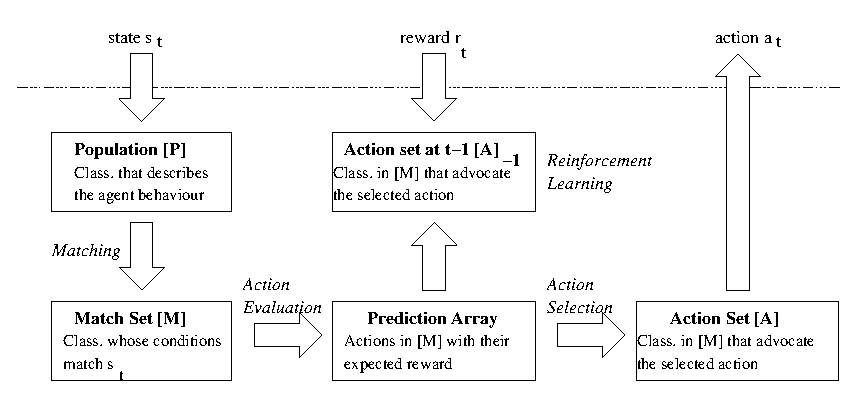
\includegraphics[scale=0.7]{images/esempio}
  \caption{\dots titolo}
  \label{fig:figura}
\end{figure}

\section{Algoritmi}
Per includere degli algoritmi come l'Algoritmo~\ref{alg:esempio}
usare lo stile \texttt{algpseudocode} presente nel package~\texttt{algorithmicx}.

%--------------------------------------------------------------------------------
% esempio di algoritmo
%--------------------------------------------------------------------------------
\begin{algorithm}[t]
  %%%
%%%
%%%	the Q-learning algorithm
%%%
%%%
\begin{algorithmic}[1]
\State Initialize $Q(\cdot,\cdot)$ arbitrarily
\ForAll{episodes}
   \State $t$ $\leftarrow$ 0
   \State Initialize $s_{t}$
   \Repeat
      \State $a_{t} \gets \pi(s_{t})$
      \State perform action $a_{t}$; observe $r_{t+1}$ and $s_{t+1}$
      \State $Q(s_{t},a_{t}) \gets Q(s_t,a_t) + \alpha( r_{t+1} + \gamma \max_{a\in A} Q(s_{t+1},a) -  Q(s_t,a_t))$
      \State $t \gets t+1$
   \Until{$s_{t}$ is terminal}
\EndFor
\end{algorithmic}

  \caption{Un esempio di algoritmo.}
  \label{alg:esempio}
\end{algorithm}


\section{Summary}

Riassunto del capitolo

%--------------------------------------------------------------------------------
% Evaluation
%--------------------------------------------------------------------------------
\chapter{Evaluation}
\label{chap:eval}
\section{Introduction}
In this chapter, in section \ref{sec:crud} will be discussed the tests used to develop the two Kundera extensions.
IN section \ref{sec:performance} will be described the YCSB framework that we have used to test the performance of the developed extensions with respect to the low level API.
Finally in section \ref{sec:data} we present the application developed to test the data synchronization capabilities of CPIM while persisting data through the Datastore Kundera extension. 

\section{Test CRUD operations}
\label{sec:crud}
The Kundera extensions development, due to the lack of information both in the documentation and from the community, has been approached in a test driven way.
The first step was then writing the required JUnit tests for the features we have planned to support.

\newparagraph We primarily want to achieve code portability of model classes, this should be exploited by the usage of the JPA interface but, as stated in chapter \ref{chap:ps}, there were problems in the old NoSQL service implementation relatively to this point.
Secondary we want to be sure that while entities are persisted in the underlying NoSQL database, they can be restored without any loss of information and thus the mapping between entities and the NoSQL database data model behave correctly in both verses.
Hence test the extensions cannot be done directly by testing single methods behavior inside the extensions code, this will for sure test the correctness of the operations but, since Kundera clients are not obliged to follow a rigid structure for their code in the implementation of the required interfaces, tests written for a client are not guaranteed to run correctly for another one. 

\noindent The approach we adopted was to define a single test suite, that will test each one of the feature we planned to support, by interacting directly with Kundera through the JPA interface. This make us able to use the same tests independently of the specific extension and thus testing the correctness of CRUD operations through the JPA interface and the portability of the code by means of tests portability.

\noindent Those tests have been primarily used to test the extensions during the development phase but they have also been executed on the remote databases instances by connecting to them through the network from the development machine. This test has been made to guarantee the correct functioning of the two extensions on real databases instance since tests runned locally are executed  against emulators of real storages.

\subsection{Tests structure}
Tests are composed by the entities, annotated with the JPA annotations, and a test class for each feature.
There are 20 defined entities that includes:
\begin{itemize}
\item simple entities related with the JPA relationships annotations, used to test relationships among entities;
\item embeddable entities and specific entities that uses those embeddable entities as data types, both types used to test the embedded feature;
\item entities with enum fields, used to test the enum fields support;
\item entities declared with different data types for the primary key identifier, used to test ids auto-generation and user-defined ids validation.
\end{itemize}

\noindent The test classes developed for testing the correctness of relationships are:
\begin{itemize}
\item \texttt{MTMTest}, to test the \textit{Many to Many} relationship type;
\item \texttt{MTOTest}, to test the \textit{Many to One} relationship type;
\item \texttt{OTMTest}, to test the \textit{One to Many} relationship type;
\item \texttt{OTOTest}, to test the \textit{One to One} relationship type;
\end{itemize}
\noindent All of those test classes implements two different methods: \texttt{testCRUD()}, that test the relationship by interacting with the method of the \texttt{EntityManager} interface, and \texttt{testQuery()}, that test the relationships by reading, updating and deleting entities through JPQL queries.

\newparagraph The remaining tests classes are:
\begin{itemize}
\item \texttt{ElementCollectionTest}, that tests the JPA feature for persisting list of entities within another one;
\item \texttt{EmbeddedTest}, that tests the JPA feature of persisting user-defined data-types as field of entities;
\item \texttt{EnumeratedTest}, that tests the JPA feature of persisting enum fields;
\item \texttt{QueryTest}, that tests the execution of various \textit{SELECT} queries and the support for the various JPQL clauses in queries.
\end{itemize}

\section{Performance tests}
\label{sec:performance}

\subsection{Yahoo Cloud Serving Benchmark}
 
\subsection{YCSB adapters}

\subsection{YCSB tests results}

\section{Hegira generator}
\label{sec:data}
To be able to test the interaction between the CPIM library and the synchronization system and to provide an example of usage of the extended CPIM library, we have developed \textit{Hegira generator}.

\noindent The application provides two behaviors through command line interface, a \texttt{clean} command to clean-up the remote Datastore instance by deleting all the entities of all Kinds, and a \texttt{generate} command that take as argument the number of entities to be generated per table and generates them.

\newparagraph Data generation is done upon a pre-defined entity model inside the application and described by the ER diagram of figure \ref{fig:hegira-generator-er}.
Build an entity generator agnostic to the entities model was not our goal and it would have required a way to automatically build the dependency graph of the entities since entities related to other ones should have a reference to the entity they depends on. Hence the application is aware of the entities dependencies and generates them accordingly.

\begin{figure}[tbh]
  \centering
  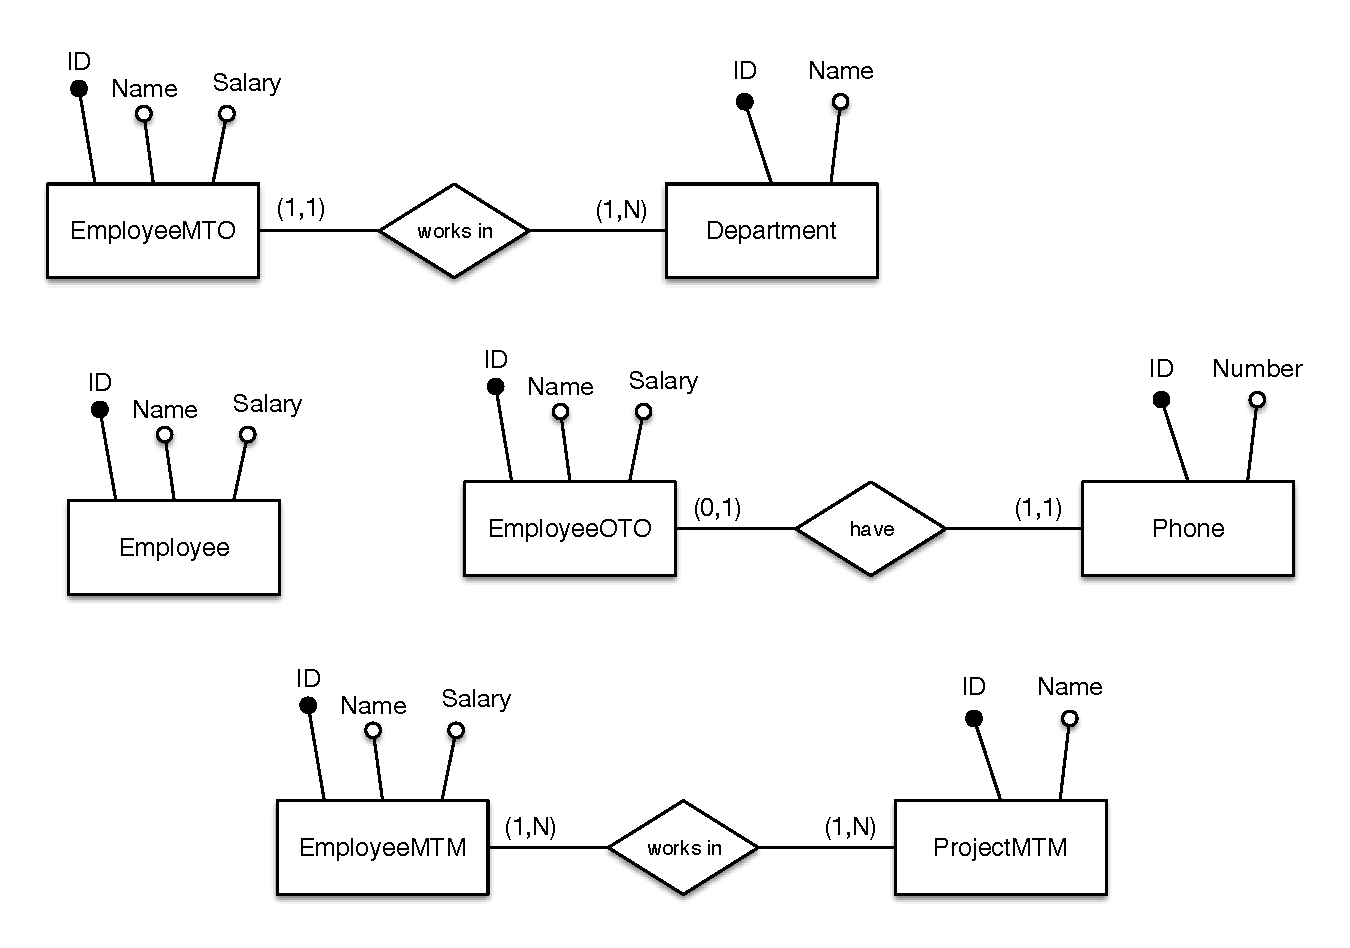
\includegraphics[width=10cm]{images/hegira_generator_er}
  \caption{ER diagram of Hegira-generator model}
  \label{fig:hegira-generator-er}
\end{figure} 

\noindent To be able to generate random entities, two methods are used:
\begin{itemize}
\item \texttt{persist(Class master)} that generates and persist entities without dependencies (such as \texttt{Employee} in the application model;
\item \texttt{persist(Class master, Class slave, DependencyType type)} that generates and persist the entities of the \textit{master} class, then uses randomly extracted entities among those just generated to fill the dependencies for the entities of the \textit{slave} class.
The \texttt{DependencyType} would be \texttt{SINGLE}, if the \textit{slave} class needs just one element to fill the dependency (which is the case of \textit{One to One} and \textit{Many to One} relationships), or \texttt{COLLECTION}, if the \textit{slave} class needs more than one element to fill the dependency (which is the case for \textit{Many to Many} relationships).
\end{itemize}

\noindent The actual entity generation is delegated to the entity itself through reflection since each entity of the model implements the \texttt{Randomizable} interface.
An example of entity genearion through this interface is shown in the snippet \ref{code:randomizable}.

\begin{lstlisting}[language=Java, caption=Entities generation, label=code:randomizable]
@Entity
public class EmployeeOTO implements Randomizable<EmployeeOTO, Phone> {
    ...
    @Override
    public EmployeeOTO randomize(Phone dependency) {
        setName(RandomUtils.randomString());
        setSalary(RandomUtils.randomLong());
        setPhone(dependency);
        return this;
    }
}
\end{lstlisting}
 
\subsection{Exploited CPIM features}
To perform the persist operation of the generated entities is used the \texttt{EntityManager} interface on which is called the \texttt{persist} method, this is completely JPA compliant and the user is not aware of what is done under the hood since communication with the synchronization system is handled automatically. An example is provided in the code \ref{code:example-persist}.

\begin{lstlisting}[language=Java, caption=Persisting entities in CPIM, label=code:example-persist]
CloudEntityManager em = MF.getFactory().getEntityManager();
Department dep = new Department("Computer Science")
em.persist(dep)
\end{lstlisting}

\noindent The persist operation through \texttt{CloudEntityManager} contacts the synchronization system to get the assigned sequence numbers for the specific tables and assign the first of them to the entity before delegating to Kundera the persist operation.

\newparagraph The application make use of the possibility of modifying at run-time the size of sequence numbers range that is requested to the synchronization system. Hence before the persist operation, the size of the sequence number range is set to the double of the number of entities to be generated. This is done through a call to \texttt{SeqNumberProvider.getInstance().setOffset(tableName, offset)}, if the resulting range size is grater than the maximum size that can be requested, is limited to that value. 

\newparagraph the last feature that is exploited by the application is the sequence number backup to file. The backup is configured in the \texttt{migration.xml} file as described in the appendix \ref{app:migration}.
This permit to the application, when is restarted, to restore the sequence numbers without the need of contacting the synchronization system.

\noindent Furthermore, to avoid execution of persist operations on a table which entities generation was completed in a previous execution, a file with the list of the table completely generated is kept in the same folder specified for the sequence numbers backup files.

\section{Summary}
In this chapter we have presented the test of correctness and performance made for the two developed Kundera extension showing the minimal performance loss that Kundera add to the low-level API.
Finally we have presented \textit{Hegira-generator}, the application developed to test the mechanisms developed inside CPIM to interacts with the synchronization system.


%--------------------------------------------------------------------------------
% Conclusions and future works
%--------------------------------------------------------------------------------
\chapter{Conclusions and future Works}
\label{chap:conclusions}
This work presented an approach of interacting with many different NoSQL databases through the CPIM library and the integration of the migration and synchronization system \textit{Hegira}.

\newparagraph The CPIM library has been modified in order to get rid of the previous implementation of the NoSQL service that was not able to guarantee full portability of the application code due to the numerous JPA implementation used to support different NoSQL databases. This work have made order in the CPIM library and added the ability for the users to interact with numerous different NoSQL solution through a common interface, identified in the JPA interface, thanks to Kundera, an open source, JPA compliant ORM for NoSQL databases.

\noindent Furthermore have been produced two brand new clients for Kundera contributing thus to the project by adding the support for Google Datastore and Azure Tables. The developed extensions has been tested in terms of throughput and latency in order to verify that the overhead added by Kundera and by its clients was not destructive for performance with respect to the use of low level API for interacting with the NoSQL databases.

\noindent The results showed that, since no significant overhead is added to the low level API version of NoSQLs, the approach we propose is worth the little loss of performance due to the great benefit it brings in terms of code portability through the CPIM library and the ability of interacting with many different NoSQL databases with a unique and well known interface.

\newparagraph The NoSQL service of CPIM library has been further modified to integrate the required logic for interacting with the migration and synchronization system \textit{Hegira}. This allows an user of the CPIM library 
 
\newparagraph Possible future works should continue on both CPIM and Kundera. Indeed, CPIM needs to be updated to interacts with the latest version of the various cloud provider API and some components needs to be rewritten, as explained in section \ref{sec:cpim-problems} for the Queue service.

\noindent Further work can also be done in intercepting the user queries, that are then sent to the migration system, supporting for example the \textit{criteria API} discussed in section \ref{sec:cpim-intercept-queries}.

\noindent Some work can be made in solving the problems that have prevented us from replicating the YCSB tests for Hbase. In this way the results presented in this work can be compared with the results of the tests performed by the Kundera team on the other clients.

\noindent Finally some work can be done in adding to Kundera the support for more NoSQL databases such as Dynamo DB.


%--------------------------------------------------------------------------------
% appendices
%--------------------------------------------------------------------------------
\part*{Appendices\label{part:app}\addcontentsline{toc}{part}{Appendices}}
\appendix
\chapter{Configuring Kundera extensions}
\label{app:kconfig}
\section{Introduction}
In this appendix are described in detail the configurations available for the two developed Kundera extensions. Are described the required properties that needs to be configured in the \textit{persistence.xml} file and the available properties that can be defined in the external datastore specific properties file.

\section{Common configuration}
The main configuration is performed in the \textit{persistence.xml} file and it follows the JPA standard.
The template of the file is as follow:

\begin{lstlisting}[language=XML, caption=persistence.xml template]
<?xml version="1.0" encoding="UTF-8" standalone="no"?>
<persistence ... >
    <persistence-unit name="...">
    <provider>com.impetus.kundera.KunderaPersistence</provider>
        <class> ... </class>
        <exclude-unlisted-classes>true</exclude-unlisted-classes>
        <properties>
            <!-- kundera properties -->
        </properties>
    </persistence-unit>
</persistence>
\end{lstlisting}

\noindent A name for the persistence unit is mandatory as it will be referenced inside the classes of the model as shown in the snippet \ref{code:class-example} in which has been declared as schema the \texttt{kundera.keyspace} property to the persistence unit name.
The full name of the classes that needs to be handled through this persistence unit must be specified in the \texttt{<class>} tag.
Each extension needs different configuration that needs to be specified inside the \texttt{<properties>} tag.

\begin{lstlisting}[language=Java, caption=Declaring the schema, label=code:class-example]
@Table(schema = "gae-test@pu")
public class Employee {

    @Id
    @Column(name = "EMPLOYEE_ID")
    private String id;

    @Column(name = "NAME")
    private String name;

    @Column(name = "SALARY")
    private Long salary;
}
\end{lstlisting}

\section{GAE Datastore}
\label{appendix:datastore-config}
Two configuration are possible:
\begin{enumerate}
\item use the datastore instance within the app engine application;
\item use a remote datastore instance through remote API.
\end{enumerate}

\newparagraph The properties to be specified inside the \texttt{<properties>} tag for the first case are:
\begin{itemize}
\item \texttt{kundera.client.lookup.class} (\textit{required}), must be set to \\ \texttt{it.polimi.kundera.client.datastore.DatastoreClientFactory};
\item \texttt{kundera.ddl.auto.prepare} (\textit{optional}), possible values are:
\begin{itemize}
\item \texttt{create}, which creates the schema (if not already exists);
\item \texttt{create-drop}, which drop the schema (if exists) and creates it;
\end{itemize}
\item \texttt{kundera.client.property} (\textit{optional}), the name of the xml file containing the datastore specific properties.
\end{itemize}

\noindent In addition to the previous properties and in case of remote API, those properties are also necessary:
\begin{itemize}
\item \texttt{kundera.nodes} (\textit{required}), url of the app engine application on which the datastore is located;
\item \texttt{kundera.port} (\textit{optional}) default is \textbf{443}, port used to connect to datastore;
\item \texttt{kundera.username} (\textit{required}), username of an admin on the remote server;
\item \texttt{kundera.password} (\textit{required}), password of an admin on the remote server.
\end{itemize}

\noindent To test against local app engine run-time emulator the configuration is as follow:

\begin{lstlisting}[language=XML, caption=GAE Datastore emulator configuration]
<property name="kundera.nodes" value="localhost"/>
<property name="kundera.port" value="8888"/>
<property name="kundera.username" value="username"/>
<property name="kundera.password" value=""/>
\end{lstlisting}

\noindent in this case the value for \texttt{kundera.password} does not matter.

\subsubsection{Datastore specific properties file}
A file with client specific properties can be created and placed inside the classpath, its name must be specified in the \textit{persistence.xml} file through the property \texttt{<property name="kundera.client.property" value="filename.xml"/>}.
The template of the file is the following:

\begin{lstlisting}[language=XML, caption=GAE Datastore - datastore specific configuration]
<?xml version="1.0" encoding="UTF-8"?>
<clientProperties>
    <datastores>
        <dataStore>
            <name>datastore</name>
            <connection>
                <properties>
                    <property name="..." value="..."></property>
                </properties>
            </connection>
        </dataStore>
    </datastores>
</clientProperties>
\end{lstlisting}

\noindent The available properties are:
\begin{itemize}
\item \texttt{datastore.policy.read} (\texttt{optional}) [eventual\textbar strong] default is \textbf{strong}. Set the read policy;
\item \texttt{datastore.deadline} (\textit{optional}). RPCs deadline in seconds;
\item \texttt{datastore.policy.transaction} (\textit{optional}) [auto\textbar none] default is \textbf{none}. Define if use implicit transaction.
\end{itemize}

\section{Azure Tables}
\label{appendix:table-config}
The properties to be specified inside the \texttt{<properties>} tag are:
\begin{itemize}
\item \texttt{kundera.username} (\textit{required}), the storage account name available from azure portal;
\item \texttt{kundera.password} (\textit{required}), the storage account key available from azure portal;
\item \texttt{kundera.client.lookup.class} (\textit{required}), must be set to\\\texttt{it.polimi.kundera.client.azuretable.AzureTableClientFactory};
\item \texttt{kundera.ddl.auto.prepare} (\textit{optional}), possible values are:
\begin{itemize}
\item \texttt{create}, which creates the schema (if not already exists);
\item \texttt{create-drop}, which drop the schema (if exists) and creates it.
\end{itemize}
\item \texttt{kundera.client.property} (\textit{optional}), the name of the xml file containing the datastore specific properties.
\end{itemize}

\subsubsection{Datastore specific properties file}
A file with client specific properties can be created and placed inside the classpath, its name must be specified in the \textit{persistence.xml} file.
The template of the file is the following:

\begin{lstlisting}[language=XML, caption=Azure Tables - datastore specific configuration]
<?xml version="1.0" encoding="UTF-8"?>
<clientProperties>
    <datastores>
        <dataStore>
            <name>azure-table</name>
            <connection>
                <properties>
                    <property name="..." value="..."></property>
                </properties>
            </connection>
        </dataStore>
    </datastores>
</clientProperties>
\end{lstlisting}

\noindent The available properties are:
\begin{itemize}
\item \texttt{table.emulator} (\textit{optional}) [true\textbar false] default is \textbf{false}. If present (and set to true) storage emulator is used. When using development server \texttt{kundera.username} and \texttt{kundera.password }in \textit{persistence.xml} are ignored;
\item \texttt{table.emulator.proxy} (\textit{optional}) default is \textbf{localhost}. If storage emulator is used set the value for the emulator proxy;
\item \texttt{table.protocol} (\textit{optional}) [http\textbar https] default is \textbf{https}. Define the protocol to be used within requests;
\item \texttt{table.partition.default} (\textit{optional}) default is \textbf{DEFAULT}.
The value for the default partition key, used when no one is specified by the user.
\end{itemize}

\chapter{Run YCSB tests}
\label{app:ycsb}
\section{Introduction}
Introduzione agli argomenti trattati nell'appendice, dalle 4 alle 10 righe.

\section{Run tests for low-level API version}
\label{appendix:ycsb-low-level}

\section{Run tests for Kundera version}
\label{appendix:ycsb-kunders}


%--------------------------------------------------------------------------------
% bibliography
%--------------------------------------------------------------------------------
\bibliographystyle{plain}
\bibliography{tesi.bib}

\end{document}
